\documentclass[sans]{beamer}

\mode<presentation>
{
	% \usetheme{CambridgeUS}
	% \usetheme{Hannover}
  \usetheme{Singapore}
	\usecolortheme{default}
}

\usepackage{cmap}
\usepackage{listings}
\usepackage{lmodern}
\usepackage{color}
\usepackage{minted}
\usepackage{graphicx}
\usepackage{tikz}
\usetikzlibrary{arrows}
\usepackage{wrapfig}

\usepackage[labelformat=empty]{caption}
\usepackage{fontspec}
\usepackage{polyglossia}
\setdefaultlanguage{russian}

\setmainfont[Ligatures=TeX]{DejaVu Serif}
\setsansfont[Ligatures=TeX]{DejaVu Sans}
\setmonofont{DejaVu Sans Mono}

\definecolor{myGray}{RGB}{50,50,50}

\begin{document}
\title
[PTOPPCC]
{Полиномиальной сложности оптимальные принтер-комбинаторы с выбором}
\author
[Подкопаев Антон]
{Подкопаев Антон, 545 группа}
\institute{
	\vspace{0.7cm}
	Научный руководитель: к.ф.-м.н. Булычев Д.Ю.
	\vspace{0.7cm}	
}
\date [12-05-14]{12 мая 2014}

\begin{frame}[plain]
	\titlepage
\end{frame}

\section{Контекст задачи}

\begin{frame}{Принтеры}
	Языковые процессоры

	\begin{block}{}
		\begin{itemize}
			\item Синтаксический анализ
			\item Преобразование
			\item Представление результата
			% Часто результат - программа на другом языке
			\begin{itemize}
				\item \textbf{Код программы}
				\item ...
			\end{itemize}
		\end{itemize}
	\end{block}
  
  \textbf{Форматирование кода в IDE}

\end{frame}

\begin{frame}{Требования на принтер}
  \begin{itemize}
    \item Соответствие стандарту кодирования
      \begin{itemize}
        \item GNU, BSD, PEP 8, Google Java Style...
      \end{itemize}
      \vfill
    \item Ограничение на ширину вывода
      \begin{itemize}
        \item 60, 80, 150 символов в строке
      \end{itemize}
      \vfill
    \item Обозримость текста
      \begin{itemize}
        \item \textbf{Оптимальное} представление занимает
          минимальное число строк
      \end{itemize}
  \end{itemize}
\end{frame}

\begin{frame}{Декларативное описание принтеров}
Задание принтеров с помощью примеров использования (эталонного кода)

\begin{columns}
  \begin{column}{0.4\linewidth}
    \begin{columns}
      \begin{column}{0.6\linewidth}
        \scriptsize
        \inputminted{java}{codes/whileEx.java}
      \end{column}
      \begin{column}{0.4\linewidth}
        Эталон
      \end{column}
    \end{columns}
    \hrule
    \vspace{1mm}
    \begin{columns}
      \begin{column}{0.6\linewidth}
        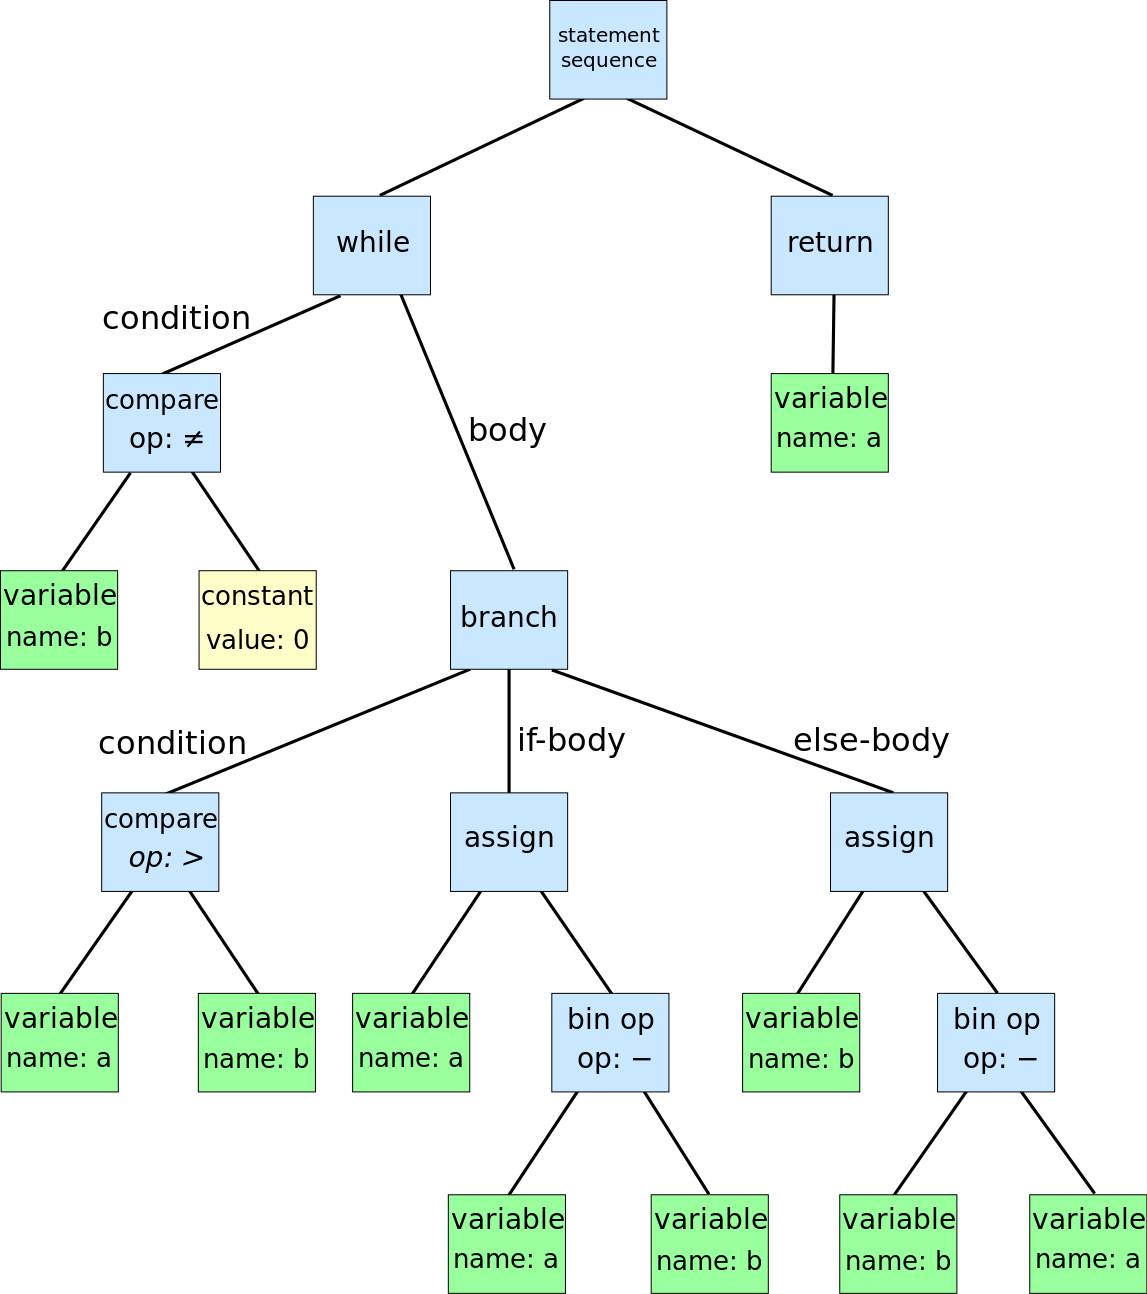
\includegraphics[width = \linewidth]{../semiPres/images/ast.png}
      \end{column}
      \begin{column}{0.4\linewidth}
        Дерево
      \end{column}
    \end{columns}

  \end{column}
  \begin{column}{0.25\linewidth}
    \scriptsize
    \inputminted{java}{codes/whileRes.java}
  \end{column}
  \begin{column}{0.1\linewidth}
    Вывод
  \end{column}
\end{columns}
\end{frame}

\begin{frame}{Принтер-комбинаторы}
  \begin{itemize}
    \item Принтер-комбинаторы --- низкоуровневые примитивы обработки блоков текста
  \end{itemize}

  \vspace{0.2cm}

  \begin{columns}
    \begin{column}{0.3\linewidth}
      \centering
      \tikz{
        \draw[line width=2pt] (0,0) -- (1,0) -- (1,0.2) -- (2,0.2) -- (2,1) -- (0, 1) -- cycle;
      }
    \end{column}
    
    \begin{column}{0.3\linewidth}
      \centering
      \tikz{
        \draw[line width=2pt] (0,0) -- (1,0) -- (1,0.2) -- (2,0.2) -- (2,1) -- (0, 1) -- cycle;
        \draw[line width=2pt]
        (1.1,-0.9) -- (2.1,-0.9) -- (2.1,-0.7) -- (3.1,-0.7) -- (3.1,0.1) -- (1.1,0.1) -- cycle;
      }
    \end{column}

    \begin{column}{0.3\linewidth}
      \centering
      \tikz{
        \draw[line width=2pt] (0,0) -- (1,0) -- (1,0.2) -- (2,0.2) -- (2,1) -- (0, 1) -- cycle;
        \draw[line width=2pt]
        (0,-1.1) -- (1,-1.1) -- (1,-0.9) -- (2,-0.9) -- (2,-0.1) -- (0,-0.1) -- cycle;
      }
    \end{column}
  \end{columns}

  \vspace{0.2cm}

  \begin{itemize}
    \item Комбинатор выбора
    \item Экспоненциальная сложность при оптимальном выводе
  \end{itemize}
\end{frame}

\section{Постановка задачи}

\begin{frame}{Постановка задачи}
  \begin{itemize}
    \item Разработать эффективную принтер-комбинаторную библиотеку,
      пригодную для реализации принтеров на шаблонах
      \vfill
    \item Апробировать метод декларативного задания принтеров для языка Java
  \end{itemize}
\end{frame}

\section{Решение}

\begin{frame}{Полиномиальные принтер-комбинаторы}
  \begin{itemize}
    \item Сведение задачи к Bottom-Up Rewrite Systems
    \item Расширение набора комбинаторов
    \item Сложность
      \begin{itemize}
        \item Было: $O(2^n)$
        \item Стало
          \begin{itemize}
            \item Стандартный набор комбинаторов: $O(w ^ 4 \times n)$
            \item Расширенный набор комбинаторов: $O(w ^ 6 \times n)$
          \end{itemize}
      \item $w$ --- ширина вывода
      \item $n$ --- размер дерева комбинаторов
      \end{itemize}
    \item Поиск минимумов по отношению частичного порядка на представлениях
  \end{itemize}
\end{frame}

\begin{frame}{Апробация задания шаблонных принтеров}
  \begin{itemize}
    \item Принтер-плагин IntelliJ IDEA для Java
    \item Получение шаблонов из эталонного репозитория
    \item Время работы: 2-4 с. для больших файлов (7-12к строк)
    \item Сложности
      \begin{itemize}
        \item Списки
        \item Комментарии
        \item Порядок у ``свободных'' поддеревьев
      \end{itemize}
    \item Реализация на Kotlin
  \end{itemize}
\end{frame}

\section{Планы и результаты}

\begin{frame}{Планы для развития}
  \begin{itemize}
    \item Анализ эталона на полноту
    \item Повышение производительности
    \item Абстрагирование метода задания шаблонных принтеров
  \end{itemize}
\end{frame}

\begin{frame}{Результаты}
  \begin{itemize}
    \small
    \item Проведено сведение задачи поиска оптимального представления к BURS
      \vfill
    \item Разработаны полиномиальной сложности оптимальные принтер-комбинаторы с выбором
      \vfill
    \item Статья о комбинаторах принята на PSI'14
      \vfill
    \item Проведена апробация подхода описания принтеров с помощью шаблонов
       в виде реализации принтер-плагина IntelliJ IDEA для языка Java
  \end{itemize}
  
\end{frame}

\end{document}
